\title{CS534 Implementation Assignment 2:\\Naive Bayes}
\author{
        Amit Bawaskar, Michael Lam\\
        EECS, Oregon State University\\
        %\email{}
        %\and
}

\documentclass[12pt]{article}
\usepackage[english]{babel}
\usepackage{graphicx}
\usepackage{subfig}
\usepackage{amsmath}
\usepackage{hyperref}
\hypersetup{
    colorlinks,%
    citecolor=green,%
    filecolor=magenta,%
    linkcolor=red,%
    urlcolor=cyan
}

%\underset{x}{\operatorname{argmax}}
%\underset{x}{\operatorname{argmin}}
\DeclareMathOperator*{\argmin}{arg\,min}
\DeclareMathOperator*{\argmax}{arg\,max}

\begin{document}
\maketitle

\begin{abstract}
In this assignment, we implemented the Naive Bayes classifier with the Bernoulli model and Multinomial model, and compared their performance.
\end{abstract}

% -------------------------------------------------
\section{Introduction}
We implemented the Naive Bayes classifier to solve a document classification problem on the 20-newsgroup dataset. Two models were implemented and compared for performance: Bernoulli model and Multinomial model.

\section{Naive Bayes}
This section provides an overview of the Naive Bayes classifier and some of our implementation details.

\subsection{Model}
A Bayes classifier model learns the prior \(p(y)\) and likelihood \(p(\textbf{x}|y)\) from the training dataset and uses Bayes rule to make inferences. In a Naive Bayes Classifier, we make the conditional independence assumption that a particular feature is unrelated to any other feature given the class label. This means that the likelihood can be computed as \(p(\textbf{x}|y) = \prod_{i=1}^d p(x_i|y)\) so there is no need to estimate the joint distribution.

Despite the naive assumptions, Naive Bayes classifiers significantly reduce overfitting and complexity. They also perform reasonably well in many applications. We will evaluate its performance on the 20-newsgroup dataset.

\subsection{Inference}
Inference is performed by using Bayes rule with the learned likelihood and prior probabilities, and using decision theory to select the class that maximizes the posterior probability. The posterior probability is proportional to the product of the likelihood and prior by Bayes rule, i.e. \(p(y|\textbf{x}) \propto p(\textbf{x}|y) p(y) \). Given features as input and the learned prior and likelihood probabilities, decision theory selects the class that maximizes the posterior probability.

In the Bernoulli model, the likelihood is given by 

\begin{align}
p(\textbf{x}|y) = \sum_{i=1}^{|V|} p_{i|y}^{x_i} (1 - p_{i|y})^{(1-x_i)}
\end{align}

where \(|V|\) is the vocabulary size, \(x_i = 1\) if the word \(i\) is present in the test document and \(x_i = 0\) otherwise.

In the Multinomial model, the likelihood is given by 

\begin{align}
p(\textbf{x}|y) = \sum_{i=1}^{|V|} p_{i|y}^{x}
\end{align}

where \(|V|\) is the vocabulary size and \(x_i\) is the number word \(i\) appearing in the test document.

\subsection{Learning}
Learning the likelihood probabilities for each feature and class is done by maximum a posterior estimation. Equivalently this amounts to applying Laplace smoothing to the maximum likelihood estimator. The prior probabilities for each class is the maximum likelihood estimator for it.

In this project, the probabilities are estimated by counting training examples with some criteria. For instance, the prior in the Bernoulli model is computed by \(p(y = k) = N_k/N\) where \(N_k\) is the number of documents with class \(k\) and \(N\) is the total number of documents. The likelihood for the Bernoulli model is computed by \(p(x_i = 1 | y = k) = N_{i|k}/N_k\), which is the fraction of documents of class \(k\) where feature (word) \(x_i\) appeared.

For the Multinomial model, the prior is computed by \(p(y = k) = W_k/W\) where \(W_k\) is the total number of words in documents with class \(k\) and \(W\) is the total number of words in all documents. The likelihood for the Multinomial model is computed by \(p(x_i | y = k) = W_{i|k}/W_k\), which is equal to the total number of word \(i\) in documents with class \(k\) divided by the total number of words in documents with class \(k\).

Note that these likelihood probabilities are adjusted by using Laplace smoothing, which is described in the next section.

\subsection{Implementation Details}
In this project we operated with the log of probabilities in order to avoid underflow issues. That is, for every multiplication and division operation, we instead used addition and subtraction of the log of the operands. We also stored the log of probabilities. For decision theory, we simply selected the class that maximizes the log of the posterior probability since the log function is a monotonically increasing function. Thus we directly operated with the log of probabilities in every circumstance.

We also applied Laplace smoothing to the likelihood probability of each feature and class in order to assign a default prior to words that have not been encountered. For the Bernoulli model, the likelihood becomes the following: \(p(x_i = 1 | y = k) = (N_{i|k}+1)/(N_k + 2)\). For the Multinomial model, the likelihood becomes the following: \(p(x_i | y = k) = (W_{i|k}+1)/(W_k + |V|)\) where \(|V|\) is the vocabulary size.

\section{Bernoulli Model}

In the Bernoulli Model, we checked if the word is present or absent in the document. The overall test accuracy for the Bernoulli model is \textbf{62.3984\%}. Figure \ref{fig:confusionmat_bern} shows the confusion matrix.

\begin{figure}[!t]
  \centering
  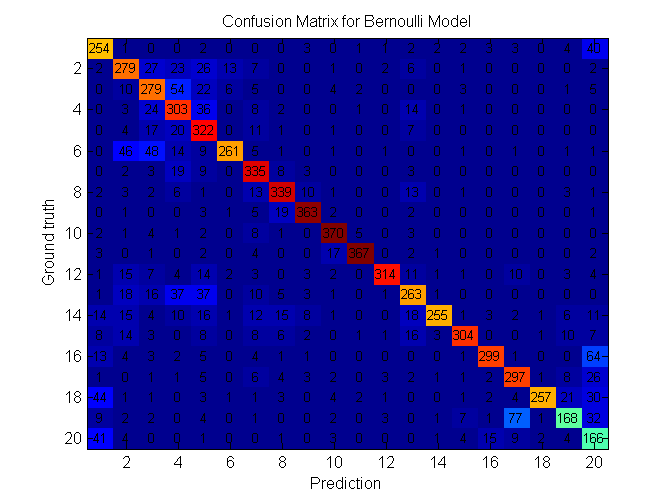
\includegraphics[scale=1]{img/confusionmat_bern.png}
  \caption{Confusion matrix for the Bernoulli model. The \(i\)th row and \(j\)th column represents the total number of times that a class \(i\) document is classified as class \(j\).}
  \label{fig:confusionmat_bern}
\end{figure}

\section{Multinomial Model}

In the Multinomial Model, instead of only looking at the presence or absence of the word, we looked at the number of times the word appeared in each document. The overall test accuracy for the Multinomial model is \textbf{77.8947\%}. Figure \ref{fig:confusionmat_multi} shows the confusion matrix. Overall the Multinomial model seems to perform better than the Bernoulli model in terms of classification accuracy.

\begin{figure}[!t]
  \centering
  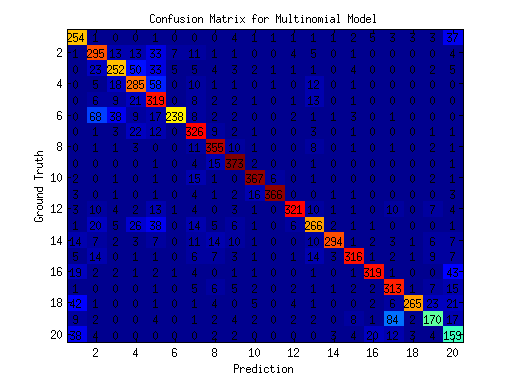
\includegraphics[scale=1]{img/confusionmat_multi.png}
  \caption{Confusion matrix for the Multinomial model. The \(i\)th row and \(j\)th column represents the total number of times that a class \(i\) document is classified as class \(j\).}
  \label{fig:confusionmat_multi}
\end{figure}

\section{Heuristics for Reducing Vocabulary Size}

We explored one heuristic for reducing the vocabulary size in hopes of improving classification accuracy. We tried eliminating words in the dictionary that have length less than or equal to a particular threshold value. We explored thresholds from 0 to 5, meaning keeping all words to keeping only words with length greater than 5.

The results in Figures \ref{fig:vocabthreshold_bern} \& \ref{fig:vocabthreshold_multi} indicate that the classification accuracy decreased as the threshold increases after 2 letters. Interestingly for the Multinomial model, accuracy increased negligibly when eliminating words up to 2 letters long. There is some intuition behind these results: it seems that words of length 3 or greater play an important role in determining the document class, while words of length 2 or fewer play a lesser role by tending to be generic English words.

\subsection{Future Work}

There are several directions for other possible heuristics. One thought is to manually create a blacklist of commonly used words to omit from the final vocabulary. The blacklist can include words such as articles, conjunctions, prepositions, etc. However, the drawback to this approach is having to manually construct this blacklist. Another thought is to calculate the average count of all the words in a document and omit those words for learning in the multinomial model that occur more than the average count. This would remove words which occur too many times in the document. It would be interesting to see if this would help or hurt performance.

\begin{figure}[!t]
  \centering
  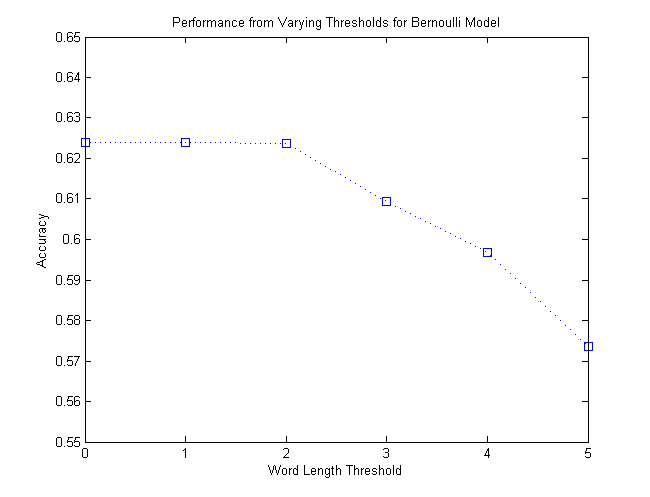
\includegraphics[scale=.60]{img/vocabthreshold_bern.png}
  \caption{Classification accuracy using the Bernoulli model and varying word length thresholds. Words of length less than or equal to the threshold value are omitted in the vocabulary for learning and inference.}
  \label{fig:vocabthreshold_bern}
\end{figure}

\begin{figure}[!t]
  \centering
  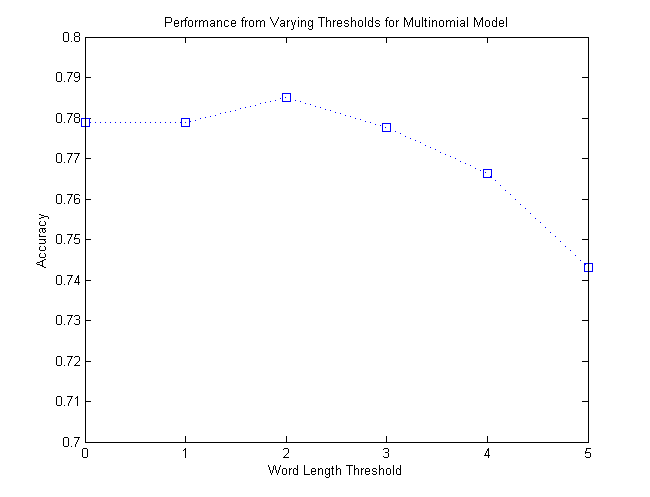
\includegraphics[scale=.60]{img/vocabthreshold_multi.png}
  \caption{Classification accuracy using the Multinomial model and varying word length thresholds. Words of length less than or equal to the threshold value are omitted in the vocabulary for learning and inference.}
  \label{fig:vocabthreshold_multi}
\end{figure}

\end{document}
This is never printed
